% !TEX root = ../main.tex

% 第一章一般名为绪论/引言,不可省略

\chapter{绪论}

\section{研究背景}

如何使计算机能够像人类一样思考、决策、行动这是人工智能科学家长久以来一直思考的问题。\cite{AIMD} 从20世纪六十年代, 科研工作者普遍关心的是如何利用计算机解决听觉、视觉、语言理解、自动推理等问题。 但是这些问题,尤其是计算机视觉和语音识别问题, 在相当长的一段时间内发展缓慢。 这是因为, 基于之前以分析为主的方法, 例如基于边缘检测等人工主观判断的特征进行图像识别, 或者利用语言学的专家知识进行语义理解和语音识别。 自从1987年, 卡内基梅隆大学李开复博士使用统计概率模型使得当时的语言识别技术大大提升, 使得人们开始注重利用统计学习模型进行人工智能相关问题的解决。 \cite{50_years_ai} \cite{manning2008introduction} \cite{abelson1985structure}

1986年, 时任加州大学圣地亚脑科学认知实验室的研究院Geoffery Hinton在Nature杂志上发表了一种利用反向传播(Back Propagation)自动优化神经网络模型的方法, 利用神经网络进行机器学习第二次成为机器学习研究的重点。 当时确实解决了一些复杂的问题, 例如1997年YaLeCun提出的卷积神经网络(Convolutional Neural Networks)能够识别手写的阿拉伯数字, 这在计算机尤其是人工智能领域是很重要的进步。 但是, 神经网络的参数多, 为了使得其参数收敛至稳定值, 需要大量的训练样本而且其巨大的矩阵运算是一般的计算机所不能承受的, 神经网络虽然有了一些优秀的表现, 但是并没有产生突破性的表现。 

2012年ImageNet计算机视觉识别比赛中,在加拿大蒙特利尔大学担任教授的Geoffery Hinton带领团队使得ImageNet图像识别的错误率由30\%以上下降到15\%一下, 这引起了轰动。 \cite{DBLP:journals/corr/abs-1301-3781} 
% htbp 什么的现在不要管
\begin{figure}[htbp]
    \centering  % 学位论文规定图表皆水平居中于版心 在 zjuthesis.cls 搜「版心设置」
    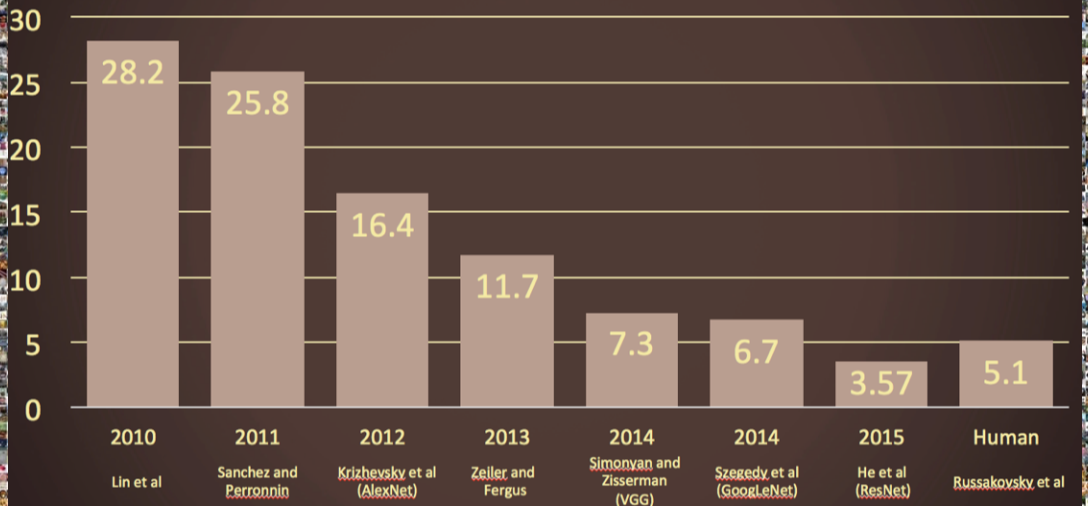
\includegraphics[width = .85\linewidth]{image_net_rank.png} % 设定图片宽度相对于版心宽度,图片文件资源名
    \caption{ImageNet 错误率的下降} % 图的题注
    \label{Russakovsky et al. arXiv, 2014} % 与 autoref 关联,设定交叉引用和显示「图x.x」
\end{figure}


从2012年之后, 深度学习这一机器学习范式, 被用来解决诸多问题。 例如此前的ImageNet下进行的计算机视觉比赛, 在2015年其识别的错误率已经低于人类的平均值。 2017年12月22日, 腾讯DPDAC NLP实验室使用深度学习神经网络训练的自然语言理解模型, 在机器阅读理解的比赛上的正确率已经达到81.790\%, 人类在这项测试中的评价准确率为\%82.304。 除计算机视觉和自然语言理解领域, 深度学习在决策领域也表现出了惊人的进步, 2017年10月, Google Deep Mind的AlphGo战胜了战胜了围棋世界排名第一的柯洁, 这表明深度学习在复杂决策上也是具有非常大的潜力。 

由于深度学习在计算机视觉、自然语言理解、决策等方面的突出表现。 科研工作者希望利用深度学习能够解决更加类似于人类的工作, 即 -- 艺术创作。 艺术创作长期以来被认为是人类独有的能力。 但是经过科学家们对于艺术创作过程以及艺术创作心理学的分析发现, 人类的艺术创作除了精神与心理学等生理原因, 其后天影响, 周围环境影响对艺术创作也是具有非常大的影响。 或者说, 创意, 创造力和后天学习具有密不可分的关系。 \cite{mq-zhanjian} \cite{adomavicius2005toward} \cite{gil2010state}


另外, 艺术创作在某些环境下也是重复的脑力活动, 例如在游戏音乐配乐, 游戏场景绘画, 电影场景绘画以及畅销书的写作等。 其重复的模式非常之多。 在此模型下, 艺术创作可以抽象为一个制作或者生成过程,如方程\eqref{eq:gene-art}所示。 

\begin{equation}\label{eq:gene-art}
ArtWork= Generator(f_0, f_1, f_2, \cdots, f_N, r_{x \sim p})
\end{equation} 

但是由于艺术生成具有区别于传统机器学习的两个特点, 第一是:其输出是一个序列性的而非特点长度的标签(Label)或者回归预测值; 第二是: 艺术的输入特征难以确定, 其输入也是一个复杂的序列过程。 例如音乐的生成依赖于诸多因素。 以上两个因素使得计算机进行自动艺术创作, 在长时间内依赖于规则,这使得计算机艺术创作不能广泛得适用于更加通用的场景。 

然而深度学习在特征自动学习(Representation Learning )和序列数据特征的提取中均具有良好的效果。 故,很多科研工作者开始使用深度学习相关的方法来尝试计算机自动生成艺术作品。 

除深度学习的背景, 《诗经》作为我国悠久的文化历史遗产。其最先即时用来歌唱的, 但是由于时间长远, 歌谱遗失。 如果能够利用现代技术为其自动谱曲, 那么将会为我国的古老艺术注入新的活力。 另外, 《诗经》虽然距离目前时代久远, 但是由于中国汉字的特点, 其大多数字义和意向与现在汉字的匹配度依然较高。 这给了使用现在歌词来恢复古老艺术的可能性。 第三, 诗经长度短小, 序列模型的长依赖问题对其影响不大, 所以也减轻了模型的训练难度。 

基于以上背景, 本文研究一种利用深度学习的理论和方法, 自动依据歌词生成音乐的方法。 并且探讨如何将其应用到诗经中。 本文提出了一种能够解决此问题的模型并使用真实数据进行了实验, 表明了该模型的有效性。 


\section{国内外研究现状}

因为本研究课题是机器学习、自然语言处理和音乐合成的交叉领域, 本小节主要从以下三方面进行国内外现状的分析: 

\begin{enumerate}

	\item 自动音乐生成
	\item 表示学习 (Representation Learning)
	\item 序列化生成 
	
\end{enumerate}

\subparagraph{计算机自动音乐生成} 实现计算机自动谱曲或者自动音乐合成不同的科研工作者使用了很不相同的方法。 考虑的范围从语法和词法等语言学知识, 到自动决策等人工智能领域的知识以及复杂系统建模等均有涉及。 目前涉及到的方法如下: 

\begin{itemize}

	\item 语言学方法
	\item 符号系统
	\item 马尔可夫链
	\item 机器学习与人工智能方法
	\item 原细胞有限自动机
	\item 基于规则的算法 [Wiggins(1991), Nierhaus(2009)]
	
\end{itemize}

%除使用以上方法, 目前仍有人工定义负责算法进行音乐的自动合成, 例如Wiggins(1991), Nierhaus(2009)。 

本文主要关注机器学习与人工智能方法的研究现状。 使用人工智能方法进行计算机自动谱曲首先提出在20世纪80年代. 1989年, Todd首先利用三层神经网络进行训练。 基于一系列初始的配置信息及已有的乐谱, 神经网络通过学习能够依据特定的配置信息(Configuration)生成特定的音高(pitch)。之后1989年, Duff使用巴赫的音乐进行训练, 是的计算机能够自动产生巴赫风格的音乐。 以上两个人使用的都是循环神经网络(Recurrent Neural Networks)。 

为了解决更加复杂的音乐合成问题, 例如节奏、旋律、和弦等, 一些研究者在人工神经网络的基础知识提出了混合系统, 即将神经网络与其他系统向结合。\cite{DBLP:ALYSIA} 较为著名的是NETNEG(Goldman et al)首先使用一个六层的神经网络产生基本的旋律片段, 然后使用基于音乐理论的规则构成的系统, 将其构成更为复杂的音乐。 该基于音乐理论的规则系统主要用于解决不同旋律之间的衔接问题。 2004年, 结合了神经网络与马尔科夫随机过程的模型被提出(Verbeurgt el al 2004)。 之后, 在2011年, Coca 等人利用神经网络加伪随机过程, 合成了能够合成较为复杂的音乐。 除此之外, 使用非监督方法也是存在的。 Burton(1998)年提出了一种生成算法模型, 首先他使用矩阵对音乐的特征进行表示, 其次其使用和弦理论,使用神经网络对不同特征进行距离。 经过这样的过程, Burton能够生成若干簇符合和弦美感的音乐。 在2007年, Phon-Amnuaisuk 等学者提出了一种新的方法。 通过音乐的自适应对应(self-organizing map)能够产生和之前所熟悉的一些音乐。 与监督学习不同的是, 该方法在产生音乐时, 并不需要训练数据。 

以上所讲述的所以生成音乐的方式全部都是面向自动产生音乐的, 使用歌词生成音乐并不如利用歌词生成音乐普遍。 Monteith等人利用已知的音乐知识, 编制了基于规则的音乐产生模型, 其通过输入文字的文字特征能够产生特定的音乐。 2016年, 加州大学圣地亚哥的Margareta Ackerman提出了一种基于随机森林的全自动音乐生成模型, 其输入为歌词, 输出为歌曲的节奏和音高(scala degree)。 虽然其模型训练结果的准确度较高, 其节奏预测的准确率达到了86.79\%, 其音高的预测准确率达到了72.28\%。 但是该模型显然有以下三个问题: 

\begin{enumerate}

\item{人工构建特征}: 该模型由人工自定义了16个特征, 包括了时间元素, 音高, 单词频率等各种。 由于人工选择特征, 不可避免的会受到人工的先验知识的影响, 并不能挖掘出深层次的范式; 
\item{训练数据过小}: 其论文使用的是24首歌进行训练, 显然该论文是音乐自动作曲的一次尝试,该结果并不能产生良好的泛化效果;
\item{输出噪声多}: 虽然该论文模型的准确率高, 但是音乐不同于其他通常的数据, 其主要在于和谐, 虽然该模型在音高上有72.28\%的准确率, 但是由于个别异常值的影响, 使得整个音乐并不具有美感。 

\end{enumerate}

但是不可否认的是, 该论文为之后利用计算机依据歌词自动生成提供了指导意义。 


\subparagraph{表示学习与Embedding} 表示学习是机器学习中重要的研究内容, 主要研究如何将数据有效的表示到计算机中。 其中, 最重要的的方式是如何通过一种方式使得新表现的数据形式能够保持其原始线性关系\cite{embedding}, 这种行为在计算机及数学中叫做embedding。Embedding是指,保持一种偏序关系,是的我们已知的某种关系也保持到新的向量空间中。 Embedding的具体定义如下:

$$ \forall x_{1},x_{2}\in X:x_{1}\leq x_{2}\Leftrightarrow F(x_{1})\leq F(x_{2}). $$


例如,之前人们对自然语言进行计算的时候, 使用的表示方式多是one-hot方法表示单词或者利用tf-idf等信息表示一句话。 但是这种表示并不能表征有效的表征句意。 Mikolov 等科学家使用的word2vec, 使得我们能够获得更加深层次的语义 \cite{DBLP:journals/corr/abs-1301-3781}。 由于word2vec保持了词汇意思的线性关系, 使得我们利用已知的单词获得新的,意思解决的单词变成了可能。 在Mikolov提出了Skip-Gram和CBOW等word Embedding的方法之后, 斯坦福大学NLP组提出的Glove,以及Salesforce提出的ContexVec \cite{DBLP:journals/corr/abs-1708-00107} 都获得更加良好的表现。 


\begin{figure}[htbp]
    \centering  % 学位论文规定图表皆水平居中于版心 在 zjuthesis.cls 搜「版心设置」
    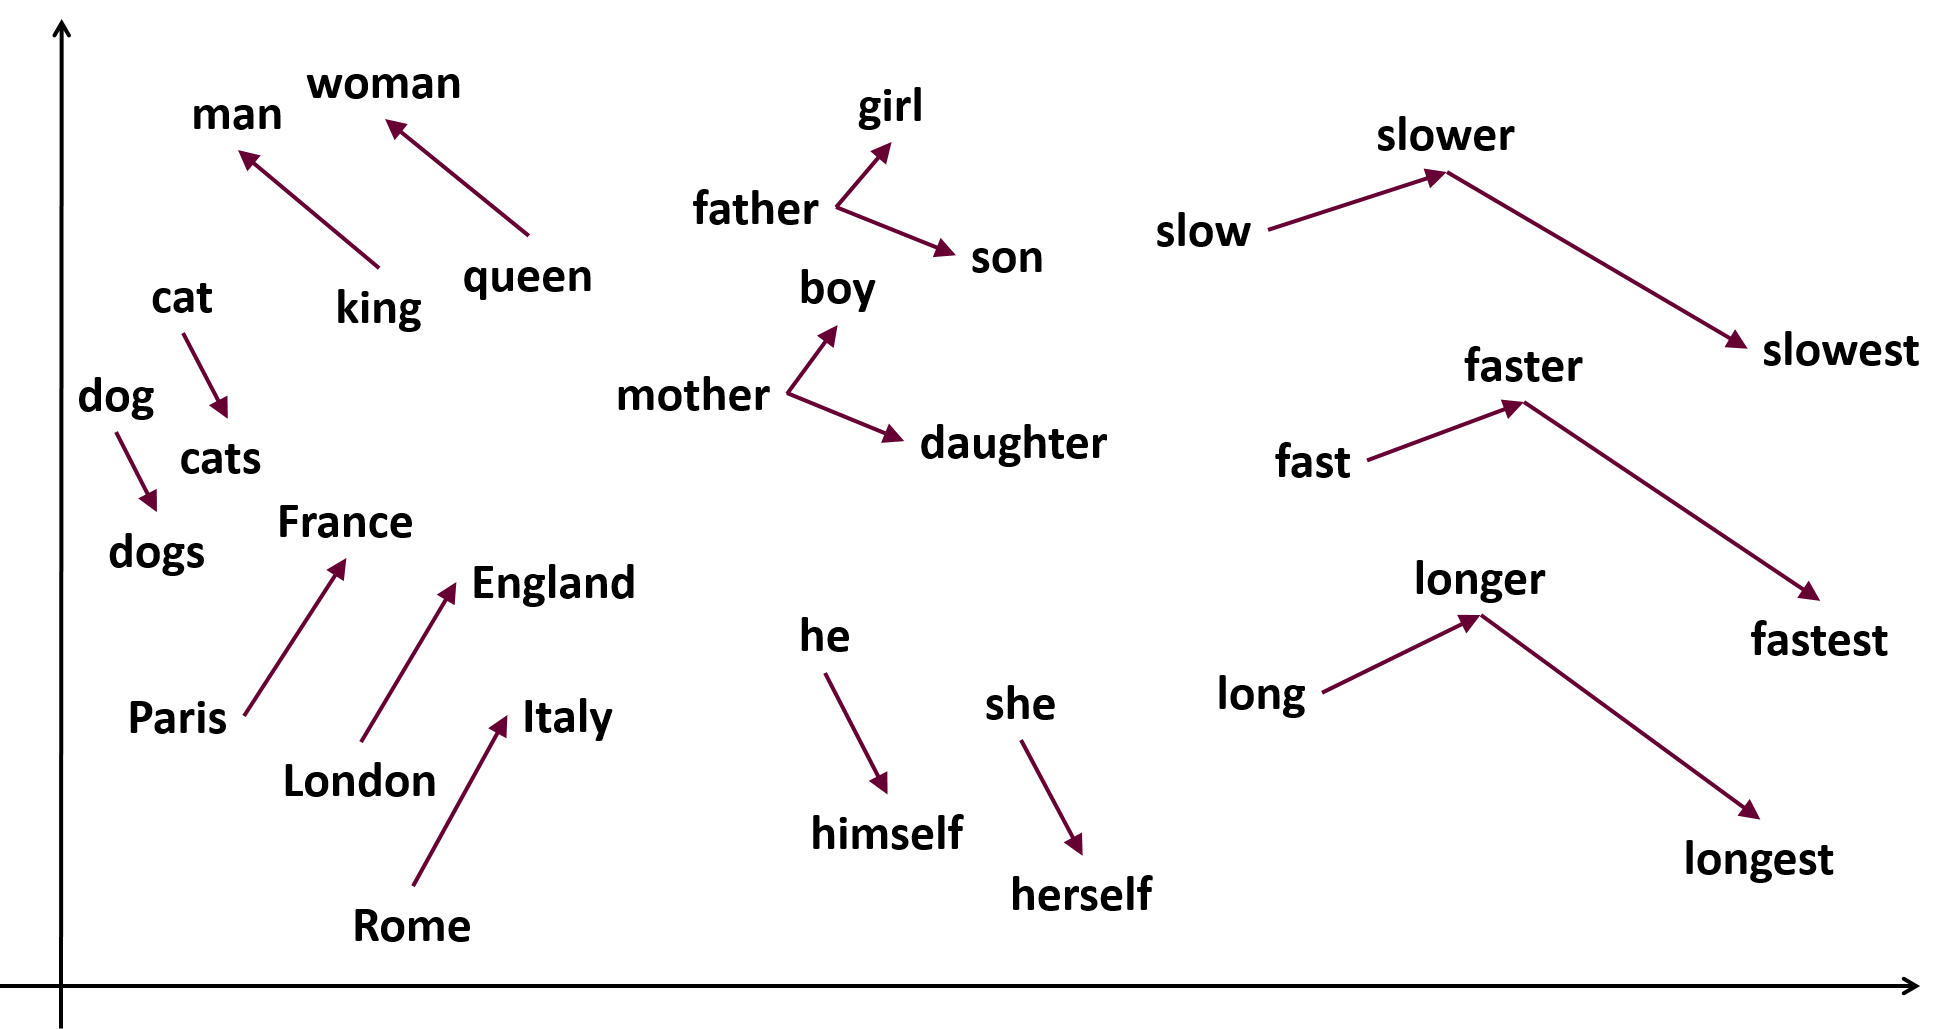
\includegraphics[width = .85\linewidth]{word2vec2.png} % 设定图片宽度相对于版心宽度,图片文件资源名
    \caption{Word Embedding 对单词词义的线性保持} % 图的题注
    \label{word2vec} % 与 autoref 关联,设定交叉引用和显示「图x.x」
\end{figure}

本文借鉴 word embedding 的思想,对音乐元素进行embedding, 这样做的好处是, 将以前的88个音乐元素扩展至用户可自定义的个数个音乐元素(依照训练数据的不同, 该自定义元素数字可从几千至几十万), 这些音乐元素经过embedding, 可使得具有类似情感,类似表达的音乐元素进行聚类。 让计算机把音乐元素当做88个单独的元素看待类似于让计算机把所有的英文文本当做26个字母看待。 经过以上关于word embdding的分析, 这显然是低效的。 如果能够让计算机自动发现类似于单词的音乐元素词组, 将能够大大提示模型的抽象能力与泛化能力。 

\subparagraph{序列化生成} 传统的机器学习模型能够处理的是输出定长的数据输出定长的预测结果。 如何使得机器学习模型能够接受边长的输入产出边长的输出, 此问题直到2014年由Google的科学家 Sutskever 等人在进行机器自动翻译模型研究时提出了Seq2Seq模型才获得了比较良好的改进 \cite{DBLP:journals/corr/SutskeverVL14}。 之后,  Bahdanau 等人又实现了在Seq2Seq模型中增加了注意力机制(Attention), 使得计算机能够接受变长输入, 输入变长的数据。 Seq2Seq以及Attention机制,使得机器翻译的水平有了大幅度的提示。 其次, Seq2Seq 也被用于自动作画, 自动生成段文字等领域。  所以本文参照机器翻译的模型, 将计算机依据歌词自动合成音乐的问题抽象为机器自动翻译的问题。


\section{论文研究内容}

文论文主要研究以下内容:

\begin{itemize}

	\item{如何获得大量的音乐训练数据}
	\item{如何高效的进行音乐元素的embedding}
	\item{如何构建序列生成模型}
	\item{如何将模型迁移适应到古代诗歌风格}

\end{itemize}

\subparagraph{如何获得大量的音乐训练数据}

利用深度学习进行序列生成首先需要解决的是大量训练数据的问题。但是面临的问题是,目前的音乐文件大多都是受版权保护的, 不能像ImageNet或者语音识别等领域具有大量的训练数据。 但是本文利用以下两种方式进行训练集的扩展: 1. 利用N-Gram以及随机skip的方式, 可能让训练数据集增加一个数量级(本文测试结果为15倍);2. 利用word embedding获得的同义词、近义词词组, 对文本进行随机替换, 可以将训练集继续增加, 增加接近一个数量级(本文实验结果为0.7倍)。经过以上两种方式, 可以将训练数据扩大两个数量级。 在下载1000首歌曲的情况下, 可以生产10万条训练记录, 基本上达到了深度学习能够利用的数据量。   

\subparagraph{如何高效的进行音乐元素的embedding}

为了更加高效的对音乐元素进行表征,本文借鉴word embedding的方式对音乐元素进行embedding。 经过这样的处理, 可以将目前常见的88个音乐元素变成更多的, 能包含具体意向、情感特征的音乐元素。 对于音乐元素单独的处理, 除了能够依据音高表示每个元素不同以外并不能包含其他的特征,但是如果能够发现更加丰富的音乐元素表示特征, 则会大大增加模型的表现能力。 也能够在情感、语义层面对其进行扩展和分析。 

但是进行高效的embedding是复杂的。 首先需要对音乐数据进行离散化处理, 虽然音乐的乐谱表现为离散值, 但是对于人类的感触是连续值。 首先需要考虑如何将音乐进行有效的离散处理。 其次是embedding时候网络结构的选择及其训练模型的定义, 网络结构如何选择, Loss函数如何定义, 这些都是本文需要考虑的问题; 第三是embedding的维度, 因为如果embedding的维度过大, 就不能在有限的数据集下收敛到到全局最优解, 如果embedding的维度过小, 就会迅速收敛到局部最小值。


\subparagraph{如何构建序列生成模型}

如何将Seq2Seq的思想利用该课题中, 即已知歌词生成乐曲, 这是本文需要解决的一个难点。 我们知道,同样的歌词可以配以不同的音乐,而同样的音乐也可以配以诸多的歌词。 例如陕北的“信天游”, 几乎所有的歌词都是一种配乐。 这就说明歌词和乐曲直接的映射关系是一种若映射, 那如何将这种弱映射关系利用模型学习出来, 是本文研究的重点。 

依据歌词生成乐曲,是不是一个可学的问题, 如果是可学的, 如何定义网络模型使得该范式可以被模型泛化, 如果不可学, 如何增加必要的辅助内容使得该范式可学, 这都是本文需要重点考虑的问题。 


\subparagraph{如何将模型迁移适应到古代诗歌风格}

本文最后采用诗经作为歌词输入,利用计算机自动为其谱曲, 但是这个具有两个问题: 一、诗经的语言形式和表现内容和用以训练的数据具有很大的不同, 如何使得模型能够适应这种语言内容, 这是需要研究的; 第二、诗经的风、雅、颂等依据史书记载, 是不同风格的。 如何做到同样类别的音乐具有类似的音乐表现, 这也是需要解决的一个难点。 

本文通过借鉴迁移学习(Transfer Learning)在计算机视觉上的成功, 在训练的Seq2Seq模型基础上对该模型进行迁移。 使模型迁移到能够适应于中国古风、诗歌;第二, 通过文本挖掘、文本分类的方法, 将不同音乐元素进行距离, 然后自动有模型得出不同音乐类型的音乐元素的分布。 之后借鉴CGAN(Conditional
 Generative Adversarial Networks)的方法, 为网络模型提供一个初始的依赖值, 通过改值用来调整音乐的美学特征。 

\section{论文组织结构}

%简明扼要的介绍下各章主旨,版面控制半页内。

\begin{itemize}

\item 第二章 \textbf{音乐元素的表征和embedding}

第二章主要解决如何将音乐元素进行有效的表征和embedding, 主要涉及到音乐元素的离散化、正则化以及标准化。 这是使得模型能够有效利用数据进行结果输出。 

\item 第三章 \textbf{歌词词向量的构建}

第三章主要利用word2vec的方法将所有的歌词进行向量化, 这是模型能够有效的使用输入训练数据进行学习。

\item 第四章 \textbf{训练数据的生成}

依据前文生成的音乐向量以及词向量, 可以此基础之上构建训练数据。 通过N-Gram滑窗, Skip-Gram随机跳跃, 以及利用word2vec结果进行同义词替换等方法, 使得模型获得了大量的训练数据。 


\item 第五章 \textbf{计算机序列生成模型的构建}

此章研究使用Seq2Seq进行序列生成的原因以及如何将Seq2Seq利用到该课题中。 主要解决此问题范式是否为可学习、可训练的问题, 以及如何使得该问题变成可学习,可训练的问题。 如何设计网络结构,层级结构, 如何选择神经元, 如何设计Loss函数, 如何设计输出输入格式, 使得该模型可训练。 

\item 第六章 \textbf{系统模型实现与结果分析}

通过网易云音乐下载的1000首歌曲, 以及通过编写网络爬虫从网络中获取到的这1000首歌曲匹配的歌词。 在此模型上进行训练,观察实验结果。 并且通过对训练结过程及结果的分析, 获得此模型的学习能力及泛化效果。 

%\item 第七章 \textbf{针对《诗经》的迁移训练}

%此章讨论如何利用迁移学习将此模型迁移到适用于《诗经》的歌曲生成中。 

\item 第七章 \textbf{总结分析}

此章讨论了此模型的优点和存在的问题, 以及提出了对未来的展望。 

\end{itemize}
